The general equation of a circle is 
\begin{align}
\implies \vec{x}^T\vec{x}+ 2\vec{u}^T\vec{x} + f = 0 \label{eq:solutions/4/2/4/2.1}
\end{align}
\begin{align}
\text{If $r$ is radius,} f =\vec{u}^T\vec{u}-r^2  \label{eq:solutions/4/2/4/2.2} \\  
  \text{center }\vec{c} =-\vec{u}
\end{align}
From equations \ref{eq:solutions/4/2/4/1.2} and \ref{eq:solutions/4/2/4/2.1},
\begin{align}
 \vec{u}  = \myvec{-3 \\ -1}\\
\implies \text{Center of the cirlce } \vec{c} = \myvec{3 \\ 1}
\end{align}
Also, radius can be determined as follows from \ref{eq:solutions/4/2/4/2.2}
\begin{align}
  \implies 8=\myvec{-3&-1}\myvec{-3\\-1}-r^2\\
  \implies 8=10 -r^2\\
  \implies r=\sqrt{2}
\end{align}
Given equation of the line is
\begin{align}
\myvec{m&-1}\vec{x}&=0 
\end{align}

It can be expressed as:-
\begin{align}
L: \quad \vec{x} = \vec{q} + \mu \vec{m} \quad \mu \in \mathbb{R} \label{eq:solutions/4/2/4/2.10} \\
\end{align}
The normal vector to the line is obtained as
\begin{align}
\vec{n} = \vec{q} + \vec{u}\\
\implies \vec{q}  = \vec{n} -  \vec{u}\\
\vec{n} =\myvec{m & -1 }^T  \text{ and } \vec{u} =\myvec{-3 & -1}^T\\
\vec{q} = \myvec{m+3 \\ 0}
\end{align}
The point $\vec{q}$ also satisfies the equation of the circle at \ref{eq:solutions/4/2/4/1.2}.
\begin{align}
\vec{q}^T\vec{q}+ 2\vec{u}^T\vec{q} + f = 0 \\
%\vec{q}^T\vec{q}-\myvec{6 &  2}\vec{q}+8 = 0 
\end{align}
\begin{multline}
(\vec{n} -\vec{ u})^T(\vec{n} -\vec{ u})+2\vec{u}^T(\vec{n} -\vec{ u})\\+f = 0
\end{multline}
\begin{multline}
\norm{\vec{n}}^2 - \vec{n}^T \vec{u} - \vec{u}^T\vec{n} + \norm{\vec{u}}^2  + 2\vec{u}^T\vec{n}\\ -2 \norm{\vec{u}}^2 +f = 0 
\end{multline}
\begin{multline}
\norm{\vec{n}}^2 - \vec{n}^T \vec{u} +\vec{n}^T\vec{u} - \norm{\vec{u}}^2  +f = 0 
\end{multline}
\begin{align}
\norm{\vec{n}}^2 - \norm{\vec{u}}^2  +f = 0\\ 
(m^2 +1) - 10 +8 = 0 \\
m^2 -1 =0\\
m=\pm 1
\end{align}
For the line \ref{eq:solutions/4/2/4/1.1} to be a tangent to circle at equation \ref{eq:solutions/4/2/4/1.2}, the values of $m$ are $\pm1$
\begin{figure}[!]
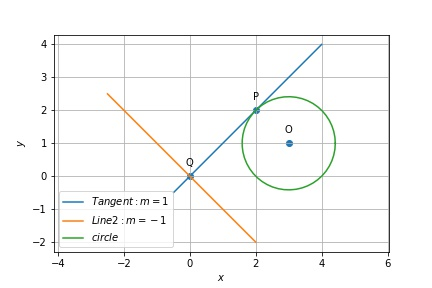
\includegraphics[width=1\columnwidth]{./solutions/4/2/4/CircleTangent.jpg}
\caption{Circle with tangent}
\label{eq:solutions/4/2/4/}
\end{figure}


